\documentclass[12pt]{article}
\usepackage{enumitem}
\usepackage{mathtools}
\usepackage{amsthm}
\usepackage{graphicx}
\graphicspath{ {images/} }
\begin{document}

\title{Assignment 11}
\author{Darwin Ding}
\maketitle

\section*{1. k-NN Rule}
\begin{enumerate}[label=(\alph*)]
	\item The following graph was created after doing cross-validation on the training set of size 300. For each odd k from 1 to 150, each point was removed and put back into the k-NN graph trained from the remaining 299 points. From here, error values were calculated and averaged to create the following graph.
	
	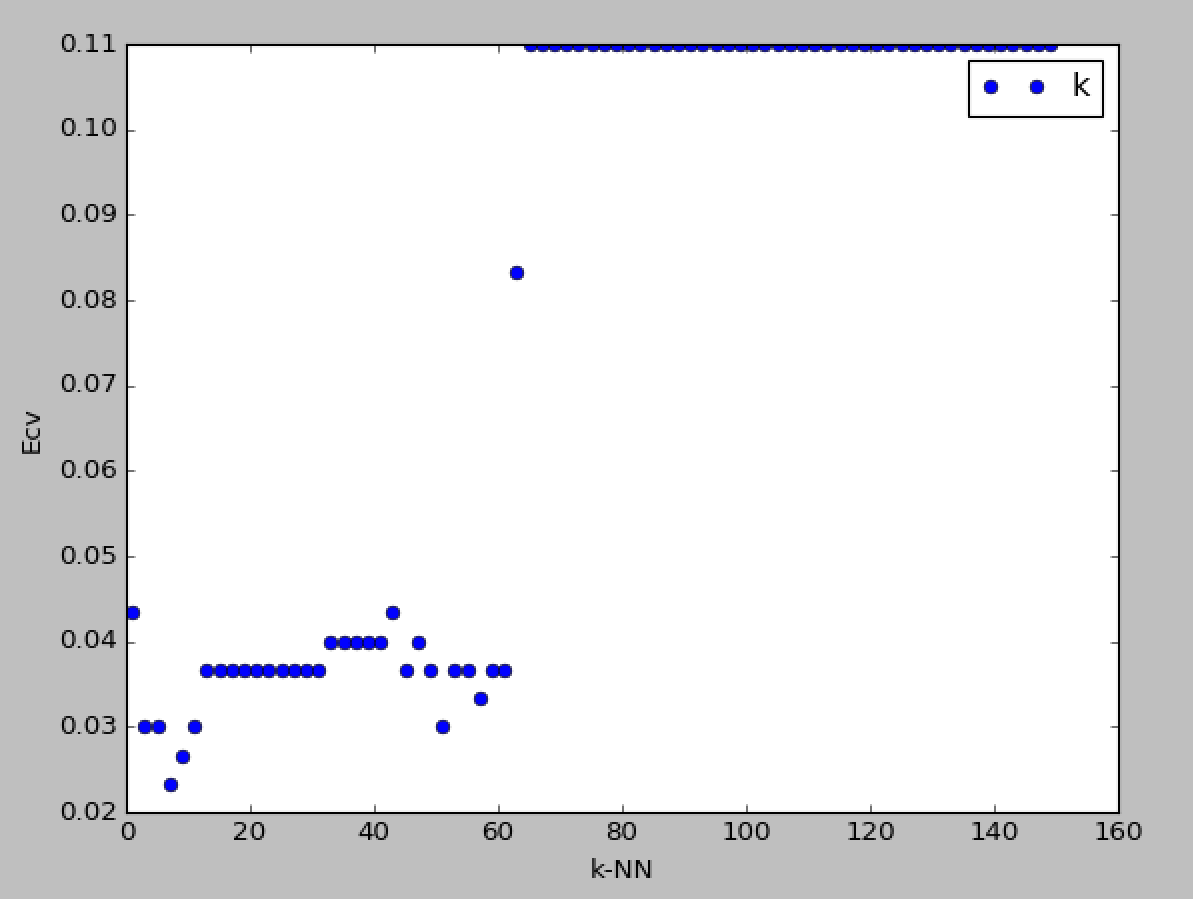
\includegraphics[scale=0.6]{1a.png}
	
	The $E_{cv}$ valleys at k = \textbf{7}, so 7-NN was selected.
	\item The $E_{cv}$ for 7-NN from the training set is \textbf{0.023}. $E_{in}$ was calculated by running each data point on the fully trained 7-NN graph. Of course, this resulted in each point being on top of its own point, but that's okay. $E_{in} = \boldsymbol{0.2}$. The decision boundary for 7-NN is displayed in the graph below:
	
	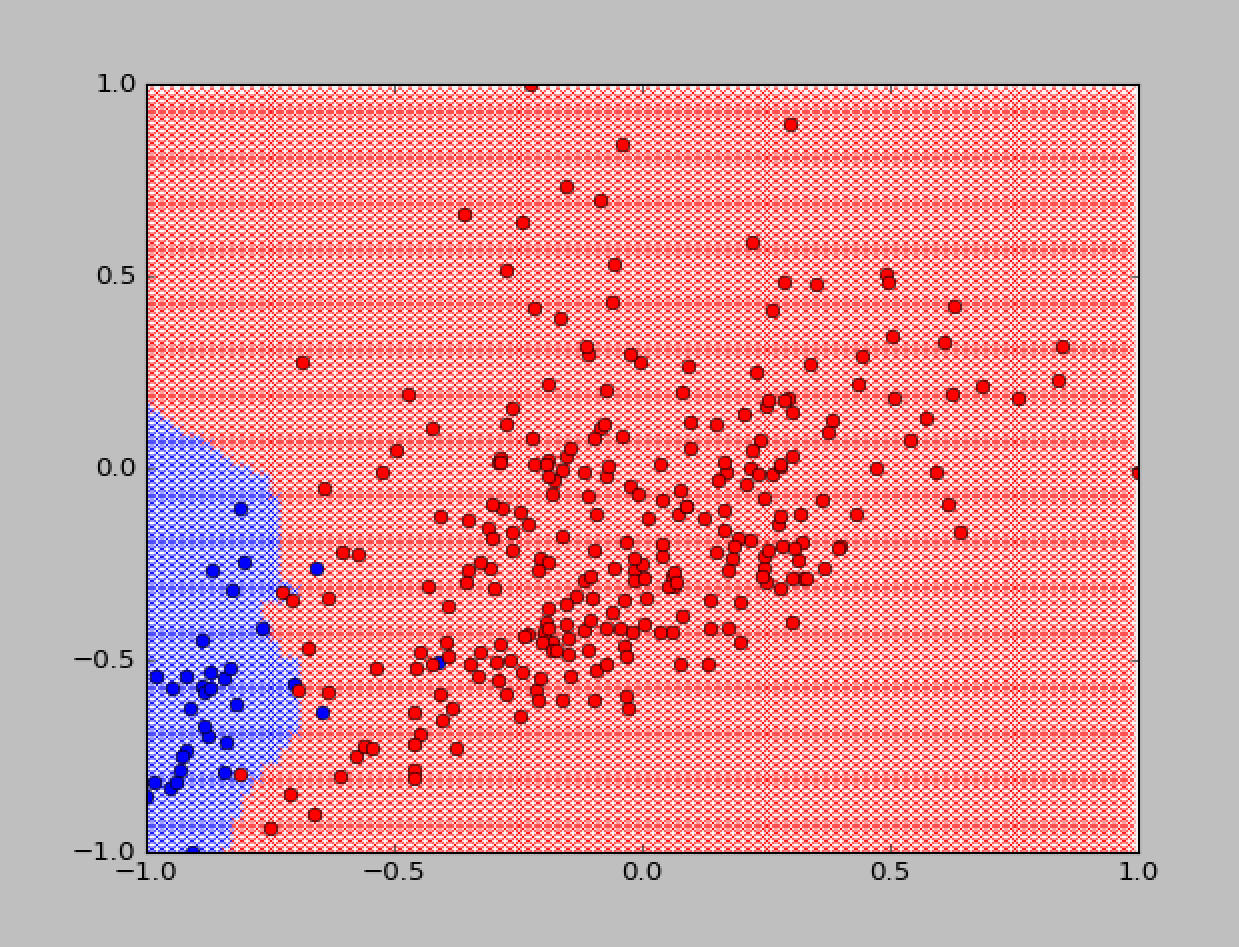
\includegraphics[scale=0.6]{1b.png}
	\item $E_{test}$ was calculated to be \textbf{0.027}. This was done by running the same 7-NN network on the remaining test points.
\end{enumerate}

\section*{2. RBF-Network}
\begin{enumerate}[label=(\alph*)]
	\item The following graph was created after doing cross-validation on the training set of size 300. For each k from 1 to 100, Lloyd's algorithm for k-means clusters was used to find k centers and the following cross-validation graph was created (after following the same algorithm described in assignment 9).
	
	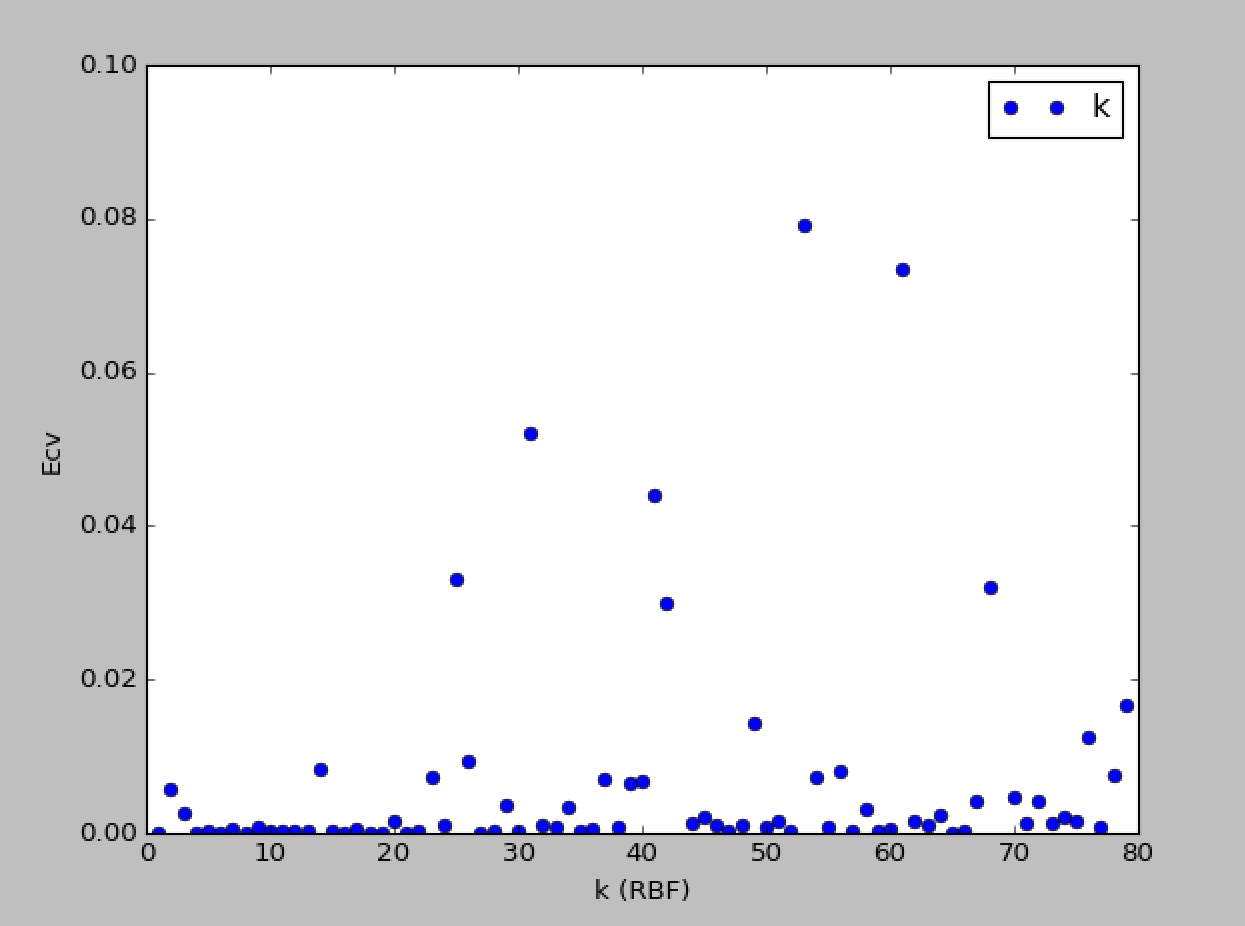
\includegraphics[scale=0.6]{2a.png}
	
	The graph valleys at k = \textbf{12} with an $E_{cv}$ of $0.016$, so $k = 12$ was selected.
	\item The $E_{in}$ was calculated to be $\boldsymbol{.18}$, which is by far and away the worst $E_{in}$ we've seen so far. I had some difficulty extracting the exact weights that the RBF was outputting, and could not display the decision boundaries.
	\item $E_{test}$ was calculated to be \textbf{0.21}. This was done by running the same RBF decision boundaries on the remaining points.
\end{enumerate}

\section*{3. Compare Linear, k-NN, RBF-Network}
The final test error after applying the straight linear model was $\boldsymbol{.0388}$. The 7-NN rule applied earlier had an $E_{test}$ of $\boldsymbol{0.027}$. The RBF-network returned a test error of $\boldsymbol{0.21}$.

Unfortunately data snooping happened in the data set when we scaled all the data points using the test set. However, we can still sort of compare the performances of each of the individual algorithms. The 7-NN rule had the smallest error, followed by the linear model and the RBF model. The 7-NN and RBF rules are, as models, significantly simpler than the linear model (which has a large multi-dimensional transform applied to it). I would probably expect the 7-NN model to have the best out of sample error. 

\end{document}